%%%%%%%%%%%%%%%%%%%%% chapter.tex %%%%%%%%%%%%%%%%%%%%%%%%%%%%%%%%%
%
% sample chapter
%
% Use this file as a template for your own input.
%
%%%%%%%%%%%%%%%%%%%%%%%% Springer-Verlag %%%%%%%%%%%%%%%%%%%%%%%%%%
%\motto{Use the template \emph{chapter.tex} to style the various elements of your chapter content.}

\chapter{Rosetta Code Tasks starting with M}

\section*{MD5}

Encode a string using an MD5 algorithm. The algorithm can be found on
\href{http://en.wikipedia.org/wiki/Md5\#Algorithm}{wikipedia}.

Optionally, validate your implementation by running all of the test
values in \href{http://tools.ietf.org/html/rfc1321}{IETF RFC (1321) for
MD5}. Additional the RFC provides more precise information on the
algorithm than the Wikipedia article.

If the solution on this page is a library solution, see
\emph{MD5/Implementation} for an implementation from scratch.

\begin{wideverbatim}

(let Str "The quick brown fox jumped over the lazy dog's back"
   (pack
      (mapcar '((B) (pad 2 (hex B)))
         (native "libcrypto.so" "MD5" '(B . 16) Str (length Str) '(NIL (16))) ) ) )

Output:

-> "E38CA1D920C4B8B8D3946B2C72F01680"

\end{wideverbatim}

\pagebreak{}
\section*{MD5/Implementation}

The purpose of this task to code and validate an implementation of the
MD5 Message Digest Algorithm by coding the algorithm directly (not using
a call to a built-in or external hashing library). For details of the
algorithm refer to
\href{http://en.wikipedia.org/wiki/Md5\#Algorithm}{MD5 on Wikipedia} or
the \href{http://www.ietf.org/rfc/rfc1321.txt}{MD5 definition in IETF
RFC (1321)}.

\begin{itemize}
\item
  The implementation needs to implement the key functionality namely
  producing a correct message digest for an input string. It is not
  necessary to mimic all of the calling modes such as adding to a digest
  one block at a time over subsequent calls.
\item
  In addition to coding and verifying your implementation, note any
  challenges your language presented implementing the solution,
  implementation choices made, or limitations of your solution.
\item
  Solutions on this page should implement MD5 directly and NOT use built
  in (MD5) functions, call outs to operating system calls or library
  routines written in other languages as is common in the original
  \emph{MD5} task.
\item
  The following are acceptable:

  \begin{itemize}
  \item
    An original implementation from the specification, reference
    implementation, or pseudo-code
  \item
    A translation of a correct implementation from another language
  \item
    A library routine in the same language; however, the source must be
    included here.
  \end{itemize}
\end{itemize}

The solutions shown here will provide practical illustrations of bit
manipulation, unsigned integers, working with little-endian data.
Additionally, the task requires an attention to details such as boundary
conditions since being out by even 1 bit will produce dramatically
different results. Subtle implementation bugs can result in some hashes
being correct while others are wrong. Not only is it critical to get the
individual sub functions working correctly, even small errors in
padding, endianness, or data layout will result in failure.

The following verification strings and hashes come from
\href{//tools.ietf.org/html/rfc1321}{RFC 1321}:

\begin{wideverbatim}
                            hash code <== string 
   0xd41d8cd98f00b204e9800998ecf8427e <== ""  
   0x0cc175b9c0f1b6a831c399e269772661 <== "a"
   0x900150983cd24fb0d6963f7d28e17f72 <== "abc"
   0xf96b697d7cb7938d525a2f31aaf161d0 <== "message digest"
   0xc3fcd3d76192e4007dfb496cca67e13b <== "abcdefghijklmnopqrstuvwxyz"
   0xd174ab98d277d9f5a5611c2c9f419d9f <== 
   "ABCDEFGHIJKLMNOPQRSTUVWXYZabcdefghijklmnopqrstuvwxyz0123456789"
   0x57edf4a22be3c955ac49da2e2107b67a <==
   "12345678901234567890123456789012345678901234567890123456789012345678901234567890"
\end{wideverbatim}

In addition, intermediate outputs to aid in developing an implementation
can be found \emph{here}.

The MD5 Message-Digest Algorithm was developed by
\href{http://en.wikipedia.org/wiki/RSA\_SecurityRSA}{RSA Data Security,
Inc.} in 1991.


\begin{wideverbatim}

This is an implementation of the pseudo-code in the Wikipedia article. Special
care had to be taken with modulo 32-bit arithmetics, as PicoLisp supports only
numbers of unspecified size.

(scl 12)
(load "@lib/math.l")  # For 'sin'

(de *Md5-R
   7 12 17 22  7 12 17 22  7 12 17 22  7 12 17 22
   5  9 14 20  5  9 14 20  5  9 14 20  5  9 14 20
   4 11 16 23  4 11 16 23  4 11 16 23  4 11 16 23
   6 10 15 21  6 10 15 21  6 10 15 21  6 10 15 21 )

(de *Md5-K
   ~(make
      (for I 64
         (link
            (/ (* (abs (sin (* I 1.0))) `(** 2 32)) 1.0) ) ) ) )

(de mod32 (N)
   (\& N `(hex "FFFFFFFF")) )

(de not32 (N)
   (x| N `(hex "FFFFFFFF")) )

(de add32 @
   (mod32 (pass +)) )

(de leftRotate (X C)
   (| (mod32 (>> (- C) X)) (>> (- 32 C) X)) )

(de md5 (Str)
   (let Len (length Str)
      (setq Str
         (conc
            (need
               (- 8 (* 64 (/ (+ Len 1 8 63) 64)))  # Pad to 64-8 bytes
               (conc
                  (mapcar char (chop Str))   # Works only with ASCII characters
                  (cons `(hex "80")) )       # '1' bit
               0 )                           # Pad with '0'
            (make
               (setq Len (* 8 Len))
               (do 8
                  (link (\& Len 255))
                  (setq Len (>> 8 Len )) ) ) ) ) )

\end{wideverbatim}

\begin{wideverbatim}

   (let
      (H0 `(hex "67452301")
         H1 `(hex "EFCDAB89")
         H2 `(hex "98BADCFE")
         H3 `(hex "10325476") )
      (while Str
         (let
            (A H0  B H1  C H2  D H3
               W (make
                  (do 16
                     (link
                        (apply |
                           (mapcar >> (0 -8 -16 -24) (cut 4 'Str)) ) ) ) ) )
               (use (Tmp F G)
                  (for I 64
                     (cond
                        ((>= 16 I)
                           (setq
                              F (| (\& B C) (\& (not32 B) D))
                              G I ) )
                        ((>= 32 I)
                           (setq
                              F (| (\& D B) (\& (not32 D) C))
                              G (inc (\& (inc (* 5 (dec I))) 15)) ) )
                        ((>= 48 I)
                           (setq
                              F (x| B C D)
                              G (inc (\& (+ 5 (* 3 (dec I))) 15)) ) )
                        (T
                           (setq
                              F (x| C (| B (not32 D)))
                              G (inc (\& (* 7 (dec I)) 15)) ) ) )
                     (setq
                        Tmp D
                        D C
                        C B
                        B
                        (add32 B
                           (leftRotate
                              (add32 A F (get *Md5-K I) (get W G))
                              (get *Md5-R I) ) )
                        A Tmp ) ) )
               (setq
                  H0 (add32 H0 A)
                  H1 (add32 H1 B)
                  H2 (add32 H2 C)
                  H3 (add32 H3 D) ) ) )
      (pack
         (make
            (for N (list H0 H1 H2 H3)
               (do 4  # Convert to little endian hex string
                  (link (pad 2 (hex (\& N 255))))
                  (setq N (>> 8 N)) ) ) ) ) ) )

\end{wideverbatim}

\begin{wideverbatim}

Output:

: (md5 "")
-> "D41D8CD98F00B204E9800998ECF8427E"
: (md5 "a")
-> "0CC175B9C0F1B6A831C399E269772661"
: (md5 "abc")
-> "900150983CD24FB0D6963F7D28E17F72"
: (md5 "message digest")
-> "F96B697D7CB7938D525A2F31AAF161D0"
: (md5 "abcdefghijklmnopqrstuvwxyz")
-> "C3FCD3D76192E4007DFB496CCA67E13B"
: (md5 "ABCDEFGHIJKLMNOPQRSTUVWXYZabcdefghijklmnopqrstuvwxyz0123456789")
-> "D174AB98D277D9F5A5611C2C9F419D9F"
: (md5 "1234567890123456789012345678901234567890
        1234567890123456789012345678901234567890")
-> "57EDF4A22BE3C955AC49DA2E2107B67A"

\end{wideverbatim}

% \pagebreak{}
% \section*{Making the application start up from a main routine}

% \begin{wideverbatim}

% PicoLisp automatically starts a REPL (read-eval-print loop), which is a kind of
% event loop. If that is not desired, call (wait), or pass -wait on the command
% line. Per convention, the GUI event loop is started by calling (go), or by
% passing -go on the command line.

% \end{wideverbatim}

\pagebreak{}
\section*{Make a backup file}

Before writing to a file it is often advisable to make a backup of the
original. Creating such a backup file is however also not without
pitfalls.

In this task you should create a backup file from an existing file and
then write new text to the old file. The following issues should be
handled:

\begin{itemize}
\item
  avoid making a copy of the file but instead rename the original and
  then write a new file with the original filename.
\item
  if a copy needs to be made, please explain why rename is not possible.
\item
  keep in mind symlinks, and do not rename or copy the link but the
  target. (If there is a link \texttt{foo -\textgreater{} bar/baz}, then
  \texttt{bar/baz} should be renamed to \texttt{bar/baz.backup} and then
  the new text should be written to \texttt{bar/baz}.)
\item
  it is assumed that you have permission to write in the target
  location, thus permission errors need not be handled.
\item
  you may choose the backup filename per preference or given
  limitations. (It should somehow include the original filename
  however.)
\item
  please try to avoid executing external commands, and especially avoid
  calling a shell script.
\end{itemize}

Some examples on this page assume that the original file already exists.
They might fail if some user is trying to create a new file.

\begin{wideverbatim}

PicoLisp makes use of external commands as much as possible (at
least for not time-critical operations), to avoid duplicated
functionality.

(let Path (in '(realpath "foo") (line T))
   (call 'mv Path (pack Path ".backup"))
   (out Path
      (prinl "This is the new file") ) )

\end{wideverbatim}

\pagebreak{}
\section*{Man or boy test}

\textbf{Background}: The \textbf{man or boy test} was proposed by
computer scientist
\href{http://en.wikipedia.org/wiki/Donald\_Knuth}{Donald Knuth} as a
means of evaluating implementations of the \emph{ALGOL 60} programming
language. The aim of the test was to distinguish compilers that
correctly implemented ``recursion and non-local references'' from
those that did not.

\begin{quote}
I have written the following simple routine, which may separate the
`man-compilers' from the `boy-compilers'\\ --- Donald Knuth
\end{quote}

\textbf{Task}: Imitate Knuth's example in Algol 60 in another language,
as far as possible.

\textbf{Details}: Local variables of routines are often kept in
\href{http://c2.com/cgi/wiki?ActivationRecord}{\emph{activation
records}} (also \emph{call frames}). In many languages, these records
are kept on a \emph{call stack}. In Algol (and e.g.
in \emph{Smalltalk}), they are allocated on a
\emph{heap} instead. Hence it is possible to pass references
to routines that still can use and update variables from their call
environment, even if the routine where those variables are declared
already returned. This difference in implementations is sometimes called
the \href{http://en.wikipedia.org/wiki/Funarg\_problem}{Funarg Problem}.

In Knuth's example, each call to \emph{A} allocates an activation record
for the variable \emph{A}. When \emph{B} is called from \emph{A}, any
access to \emph{k} now refers to this activation record. Now \emph{B} in
turn calls \emph{A}, but passes itself as an argument. This argument
remains bound to the activation record. This call to \emph{A} also
``shifts'' the variables \emph{x\textsubscript{i}} by one place, so
eventually the argument \emph{B} (still bound to its particular
activation record) will appear as \emph{x4} or \emph{x5} in a call to
\emph{A}. If this happens when the expression \emph{x4 + x5} is
evaluated, then this will again call \emph{B}, which in turn will update
\emph{k} in the activation record it was originally bound to. As this
activation record is shared with other instances of calls to \emph{A}
and \emph{B}, it will influence the whole computation.

So all the example does is to set up a convoluted calling structure,
where updates to \emph{k} can influence the behavior in completely
different parts of the call tree.

Knuth used this to test the correctness of the compiler, but one can of
course also use it to test that other languages can emulate the Algol
behavior correctly. If the handling of activation records is correct,
the computed value will be −67.

\textbf{Performance and Memory}: Man or Boy is intense and can be pushed
to challenge any machine. Memory not CPU time is the constraining
resource as the recursion creates a proliferation activation records
which will quickly exhaust memory and present itself through a stack
error. Each language may have ways of adjusting the amount of memory or
increasing the recursion depth. Optionally, show how you would make such
adjustments.

The table below shows the result, call depths, and total calls for a
range of k:

\begin{table}[H]
  \centering
  \begin{tabular}{rrrrrr}
\emph{k} & \emph{A} & \emph{A called} & \emph{A depth} & \emph{B called} & \emph{B depth} \\               
\hline{}
0 & 1 & 1 & 1 & 0 & 0 \\      
1 & 0 & 2 & 2 & 1 & 1 \\      
2 & -2 & 3 & 3 & 2 & 2 \\       
3 & 0 & 4 & 4 & 3 & 3 \\       
4 & 1 & 8 & 8 & 7 & 7 \\       
5 & 0 & 18 & 16 & 17 & 15 \\     
6 & 1 & 38 & 32 & 37 & 31 \\     
7 & -1 & 80 & 64 & 79 & 63 \\     
8 & -10 & 167 & 128 & 166 & 127 \\    
9 & -30 & 347 & 256 & 346 & 255 \\    
10 & -67 & 722 & 512 & 721 & 511 \\    
11 & -138 & 1,509 & 1,024 & 1,508 & 1,023 \\  
12 & -291 & 3,168 & 2,048 & 3,167 & 2,047 \\  
13 & -642 & 6,673 & 4,096 & 6,672 & 4,095 \\  
14 & -1,446 & 14,091 & 8,192 & 14,090 & 8,191 \\  
15 & -3,250 & 29,825 & 16,384 & 29,824 & 16,383 \\ 
16 & -7,244 & 63,287 & 32,768 & 63,286 & 32,767 \\ 
17 & -16,065 & 134,652 & 65,536 & 134,651 & 65,535 \\ 
18 & -35,601 & 287,264 & 131,072 & 287,263 & 131,071 \\
19 & -78,985 & 614,442 & 262,144 & 614,441 & 262,143 \\
20 & -175,416 & 1,317,533 & 524,288 & 1,317,532 & 524,287 \\
21 & -389,695 & 2,831,900 & 1,048,57 & 2,831,899 & 1,048,57 \\
22 & -865,609 & 6,100,852 & 2,097,15 & 6,100,851 & 2,097,15 \\ 
23 & -1,922,362 & 13,172,23 & 4,194,30 & 13,172,23 & 4,194,30 \\
24 & -4,268,854 & ~ & ~ & ~ & ~ \\      
25 & -9,479,595 & ~ & ~ & ~ & ~ \\      
26 & -21,051,458 & ~ & ~ & ~ & ~ \\      
27 & -46,750,171 & ~ & ~ & ~ & ~ \\      
28 & -103,821,058 & ~ & ~ & ~ & ~ \\      
29 & -230,560,902 & ~ & ~ & ~ & ~ \\      
30 & -512,016,658 & ~ & ~ & ~ & ~ \\      
  \end{tabular}
\end{table}


\begin{wideverbatim}

As PicoLisp uses exclusively shallow dynamic binding, stack frames have to be
explicitly constructed.

(de a (K X1 X2 X3 X4 X5)
   (let (@K (cons K)  B (cons))  # Explicit frame
      (set B
         (curry (@K B X1 X2 X3 X4) ()
            (a (dec @K) (car B) X1 X2 X3 X4) ) )
      (if (gt0 (car @K)) ((car B)) (+ (X4) (X5))) ) )

(a 10 '(() 1) '(() -1) '(() -1) '(() 1) '(() 0))

Output:

-> -67

\end{wideverbatim}

\pagebreak{}
\section*{Mandelbrot set}

Generate and draw the
\href{http://en.wikipedia.org/wiki/Mandelbrot\_set}{Mandelbrot set}.
Note that there are
\href{http://en.wikibooks.org/wiki/Fractals/Iterations\_in\_the\_complex\_plane/Mandelbrot\_set}{many
algorithms} to draw Mandelbrot set and there are
\href{http://en.wikibooks.org/wiki/Pictures\_of\_Julia\_and\_Mandelbrot\_sets}{many
functions} which generate it .

\begin{wideverbatim}

(scl 6)

(let Ppm (make (do 300 (link (need 400))))
   (for (Y . Row) Ppm
      (for (X . @) Row
         (let (ZX 0  ZY 0  CX (*/ (- X 250) 1.0 150)  CY (*/ (- Y 150) 1.0 150)  C 570)
            (while (and (> 4.0 (+ (*/ ZX ZX 1.0) (*/ ZY ZY 1.0))) (gt0 C))
               (let Tmp (- (*/ ZX ZX 1.0) (*/ ZY ZY 1.0) (- CX))
                  (setq
                     ZY (+ (*/ 2 ZX ZY 1.0) CY)
                     ZX Tmp ) )
               (dec 'C) )
            (set (nth Ppm Y X) (list 0 C C)) ) ) )
   (out "img.ppm"
      (prinl "P6")
      (prinl 400 " " 300)
      (prinl 255)
      (for Y Ppm (for X Y (apply wr X))) ) )

\end{wideverbatim}

\pagebreak{}
\section*{Map range}

Given two
\href{http://en.wikipedia.org/wiki/Interval\_(mathematics)}{ranges},
{[}\emph{a}\textsubscript{1},\emph{a}\textsubscript{2}{]} and
{[}\emph{b}\textsubscript{1},\emph{b}\textsubscript{2}{]}; then a value
\emph{s} in range
{[}\emph{a}\textsubscript{1},\emph{a}\textsubscript{2}{]} is linearly
mapped to a value \emph{t} in range
{[}\emph{b}\textsubscript{1},\emph{b}\textsubscript{2}{]} when:

\begin{figure}[H]
\centering
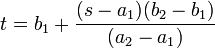
\includegraphics[scale=.6]{graphics/864ab514eca1fb4403576eb20ee0cb22.png}
% \caption{t = b\_1 + \{(s - a\_1)(b\_2 - b\_1) \textbackslash{}over (a\_2
% - a\_1)\}}
\end{figure}

The task is to write a function/subroutine/\ldots{} that takes two
ranges and a real number, and returns the mapping of the real number
from the first to the second range. Use this function to map values from
the range \texttt{{[}0, 10{]}} to the range \texttt{{[}-1, 0{]}}.

\textbf{Extra credit:} Show additional idiomatic ways of performing the
mapping, using tools available to the language.


\begin{wideverbatim}

(scl 1)

(de mapRange (Val A1 A2 B1 B2)
   (+ B1 (*/ (- Val A1) (- B2 B1) (- A2 A1))) )


(for Val (range 0 10.0 1.0)
   (prinl
      (format (mapRange Val 0 10.0 -1.0 0) *Scl) ) )

Output:

-1.0
-0.9
-0.8
-0.7
-0.6
-0.5
-0.4
-0.3
-0.2
-0.1
0.0

\end{wideverbatim}

\pagebreak{}
\section*{Matrix multiplication}

Multiply two matrices together. They can be of any dimensions, so long
as the number of columns of the first matrix is equal to the number of
rows of the second matrix.


\begin{wideverbatim}

(de matMul (Mat1 Mat2)
   (mapcar
      '((Row)
         (apply mapcar Mat2
            '(@ (sum * Row (rest))) ) )
      Mat1 ) )

(matMul
   '((1 2 3) (4 5 6))
   '((6 -1) (3 2) (0 -3)) )

Output:

-> ((12 -6) (39 -12))

\end{wideverbatim}

\pagebreak{}
\section*{Matrix transposition}

\href{http://en.wikipedia.org/wiki/Transpose}{Transpose} an arbitrarily
sized rectangular
\href{http://en.wikipedia.org/wiki/Matrix\_(mathematics)}{Matrix}.


\begin{wideverbatim}

(de matTrans (Mat)
   (apply mapcar Mat list) )

(matTrans '((1 2 3) (4 5 6)))

Output:

-> ((1 4) (2 5) (3 6))

\end{wideverbatim}

\pagebreak{}
\section*{Matrix-exponentiation operator}

Most programming languages have a built-in implementation of
exponentiation for integers and reals only.

Demonstrate how to implement matrix exponentiation as an operator.


\begin{wideverbatim}

Uses the 'matMul' function from [[Matrix multiplication#PicoLisp]]

(de matIdent (N)
   (let L (need N (1) 0)
      (mapcar '(() (copy (rot L))) L) ) )

(de matExp (Mat N)
   (let M (matIdent (length Mat))
      (do N
         (setq M (matMul M Mat)) )
      M ) )

(matExp '((3 2) (2 1)) 3)

Output:

-> ((55 34) (34 21))

\end{wideverbatim}

\pagebreak{}
\section*{Maze generation}

Generate and show a maze, using the simple
\href{http://en.wikipedia.org/wiki/Maze\_generation\_algorithm\#Depth-first\_search}{Depth-first
  search} algorithm.

\begin{enumerate}
\item
  Start at a random cell.
\item
  Mark the current cell as visited, and get a list of its neighbors. For
  each neighbor, starting with a randomly selected neighbor:

  If that neighbor hasn't been visited, remove the wall between this
  cell and that neighbor, and then recurse with that neighbor as the
  current cell.
\end{enumerate}

See also \emph{Maze solving}.


\begin{wideverbatim}

This solution uses 'grid' from "lib/simul.l" to generate the two-dimensional
structure.

(load "@lib/simul.l")

(de maze (DX DY)
   (let Maze (grid DX DY)
      (let Fld (get Maze (rand 1 DX) (rand 1 DY))
         (recur (Fld)
            (for Dir (shuffle '((west . east) (east . west)
                                (south . north) (north . south) ) )
               (with ((car Dir) Fld)
                  (unless (or (: west) (: east) (: south) (: north))
                     (put Fld (car Dir) This)
                     (put This (cdr Dir) Fld)
                     (recurse This) ) ) ) ) )
      (for (X . Col) Maze
         (for (Y . This) Col
            (set This
               (cons
                  (cons
                     (: west)
                     (or
                        (: east)
                        (and (= Y 1) (= X DX)) ) )
                  (cons
                     (: south)
                     (or
                        (: north)
                        (and (= X 1) (= Y DY)) ) ) ) ) ) )
      Maze ) )

(de display (Maze)
   (disp Maze 0 '((This) "   ")) )

\end{wideverbatim}

\begin{wideverbatim}


Output:

: (display (maze 11 8))
   +   +---+---+---+---+---+---+---+---+---+---+
 8 |           |       |                       |
   +   +   +   +   +   +   +---+   +---+---+   +
 7 |   |   |       |   |   |       |       |   |
   +---+   +---+---+   +   +   +---+   +   +   +
 6 |   |       |       |   |           |   |   |
   +   +---+   +---+   +---+---+---+   +   +---+
 5 |       |       |               |   |       |
   +---+   +---+   +---+---+---+   +---+---+   +
 4 |   |       |       |       |   |           |
   +   +---+   +---+   +---+   +   +   +---+   +
 3 |       |       |   |       |   |       |   |
   +   +---+---+   +   +   +   +   +---+   +   +
 2 |       |       |   |   |   |   |       |   |
   +   +   +   +---+   +   +---+   +   +---+   +
 1 |   |               |               |
   +---+---+---+---+---+---+---+---+---+---+---+
     a   b   c   d   e   f   g   h   i   j   k

\end{wideverbatim}

\pagebreak{}
\section*{Maze solving}

For a maze generated by \emph{this task}, write a function that finds
(and displays) the shortest path between two cells. Note that because
these mazes are generated by the
\href{http://en.wikipedia.org/wiki/Maze\_generation\_algorithm\#Depth-first\_search}{Depth-first
  search} algorithm, they contain no circular paths, and a simple
depth-first tree search can be used.

\begin{wideverbatim}

(de shortestPath (Goal This Maze)
   (let (Path NIL  Best NIL  Dir " > ")
      (recur (This Path Dir)
         (when (and This (not (: mark)))
            (push 'Path (cons This Dir))
            (if (== Goal This)
               (unless (and Best (>= (length Path) (length Best)))
                  (setq Best Path) )
               (=: mark T)
               (recurse (: west) Path " > ")
               (recurse (: east) Path " < ")
               (recurse (: south) Path " \^ ")
               (recurse (: north) Path " v ")
               (=: mark NIL) ) ) )
      (disp Maze 0
         '((Fld) (if (asoq Fld Best) (cdr @) "   ")) ) ) )

Using the maze produced in [[Maze generation#PicoLisp]], this finds the shortest
path from the top-left cell 'a8' to the bottom-right exit 'k1':

: (shortestPath 'a8 'k1 (maze 11 8))
   +   +---+---+---+---+---+---+---+---+---+---+
 8 | >   >   v | >   v |                       |
   +   +   +   +   +   +   +---+   +---+---+   +
 7 |   |   | >   ^ | v |   |       |       |   |
   +---+   +---+---+   +   +   +---+   +   +   +
 6 |   |       |     v |   |           |   |   |
   +   +---+   +---+   +---+---+---+   +   +---+
 5 |       |       | >   >   >   v |   |       |
   +---+   +---+   +---+---+---+   +---+---+   +
 4 |   |       |       |       | v | >   >   v |
   +   +---+   +---+   +---+   +   +   +---+   +
 3 |       |       |   |       | v | ^   < | v |
   +   +---+---+   +   +   +   +   +---+   +   +
 2 |       |       |   |   |   | v | >   ^ | v |
   +   +   +   +---+   +   +---+   +   +---+   +
 1 |   |               |         >   ^ |     >
   +---+---+---+---+---+---+---+---+---+---+---+
     a   b   c   d   e   f   g   h   i   j   k

\end{wideverbatim}

\pagebreak{}
\section*{Median filter}

The median filter takes in the neighbourhood the median color (see
\href{http://en.wikipedia.org/wiki/Median\_filter}{Median filter})

\emph{(to test the function below, you can use these \emph{input} and
  \emph{output} solutions)}


\begin{wideverbatim}

(de ppmMedianFilter (Radius Ppm)
   (let Len (inc (* 2 Radius))
      (make
         (chain (head Radius Ppm))
         (for (Y Ppm  T  (cdr Y))
            (NIL (nth Y Len)
               (chain (tail Radius Y)) )
            (link
               (make
                  (chain (head Radius (get Y (inc Radius))))
                  (for (X (head Len Y) T)
                     (NIL (nth X 1 Len)
                        (chain (tail Radius (get X (inc Radius)))) )
                     (link
                        (cdr
                           (get
                              (sort
                                 (mapcan
                                    '((Y)
                                       (mapcar
                                          '((C)
                                             (cons
                                                (+
                                                   (* (car C) 2126)     # Red
                                                   (* (cadr C) 7152)    # Green
                                                   (* (caddr C) 722) )  # Blue
                                                C ) )
                                          (head Len Y) ) )
                                    X ) )
                              (inc Radius) ) ) )
                     (map pop X) ) ) ) ) ) ) )

Test using 'ppmRead' from [[Bitmap/Read a PPM file#PicoLisp]] and 'ppmWrite'
from [[Bitmap/Write a PPM file#PicoLisp]]:

(ppmWrite (ppmMedianFilter 2 (ppmRead "Lenna100.ppm")) "a.ppm")

\end{wideverbatim}

\pagebreak{}
\section*{Memory allocation}

Show how to explicitly allocate and deallocate blocks of memory in your
language. Show access to different types of memory (i.e.,
\emph{heap}, \emph{stack}, shared,
foreign) if applicable.


\begin{wideverbatim}

Only the heap can be explicitly controlled in PicoLisp. Usually this is not
necessary, as it happens automatically.

But if desired, memory can be pre-allocated by calling gc with a single numeric
argument, specifying the desired number of megabytes that should be reserved.
When that argument is zero, the heap size is decreased (as far as possible).

\end{wideverbatim}

\pagebreak{}
\section*{Memory layout of a data structure}

It is often useful to control the memory layout of fields in a data
structure to match an interface control definition, or to interface with
hardware. Define a data structure matching the RS-232 Plug Definition.
Use the 9-pin definition for brevity.

\begin{verbatim}
Pin Settings for Plug
(Reverse order for socket.)
__________________________________________
1  2  3  4  5  6  7  8  9  10 11 12 13
14 15 16 17 18 19 20 21 22 23 24 25
_________________
1  2  3  4  5
6  7  8  9
25 pin                        9 pin
1 - PG   Protective ground
2 - TD   Transmitted data     3
3 - RD   Received data        2
4 - RTS  Request to send      7
5 - CTS  Clear to send        8
6 - DSR  Data set ready       6
7 - SG   Signal ground        5
8 - CD   Carrier detect       1
9 - + voltage (testing)
10 - - voltage (testing)
11 -
12 - SCD  Secondary CD
13 - SCS  Secondary CTS
14 - STD  Secondary TD
15 - TC   Transmit clock
16 - SRD  Secondary RD
17 - RC   Receiver clock
18 -
19 - SRS  Secondary RTS            
20 - DTR  Data terminal ready      4
21 - SQD  Signal quality detector
22 - RI   Ring indicator           9
23 - DRS  Data rate select
24 - XTC  External clock
25 -
\end{verbatim}



\begin{wideverbatim}

PicoLisp can handle bit fields or bit structures only as bignums. They can be
manipulated with '[http://software-lab.de/doc/ref_.html#\& \&]',
'[http://software-lab.de/doc/ref_.html#| |]' and
'[http://software-lab.de/doc/refX.html#x| x|]',
or tested with '[http://software-lab.de/doc/refB.html#bit? bit?]'.

# Define bit constants
(for (N . Mask) '(CD RD TD DTR SG DSR RTS CTS RI)
   (def Mask (>> (- 1 N) 1)) )

# Test if Clear to send
(when (bit? CTS Data)
   ... )

\end{wideverbatim}

\pagebreak{}
\section*{Menu}

Given a list containing a number of strings of which one is to be
selected and a prompt string, create a function that:

\begin{itemize}
\item
  Print a textual menu formatted as an index value followed by its
  corresponding string for each item in the list.
\item
  Prompt the user to enter a number.
\item
  Return the string corresponding to the index number.
\end{itemize}

The function should reject input that is not an integer or is an out of
range integer index by recreating the whole menu before asking again for
a number. The function should return an empty string if called with an
empty list.

For test purposes use the four phrases: ``\texttt{fee fie}'',
``\texttt{huff and puff}'', ``\texttt{mirror mirror}'' and
``\texttt{tick tock}'' in a list.

Note: This task is fashioned after the action of the
\href{http://www.softpanorama.org/Scripting/Shellorama/Control\_structures/select\_statements.shtml}{Bash
  select statement}.

\begin{wideverbatim}

(de choose (Prompt Items)
   (use N
      (loop
         (for (I . Item) Items
            (prinl I ": " Item) )
         (prin Prompt " ")
         (NIL (setq N (in NIL (read))))
         (T (>= (length Items) N 1) (get Items N)) ) ) )

(choose "Which is from the three pigs?"
   '("fee fie" "huff and puff" "mirror mirror" "tick tock") )

Output:

1: fee fie
2: huff and puff
3: mirror mirror
4: tick tock
Which is from the three pigs? 2
-> "huff and puff"

\end{wideverbatim}

\pagebreak{}
\section*{Metaprogramming}


Name and briefly demonstrate any support your language has for
metaprogramming. Your demonstration may take the form of
cross-references to other tasks on Rosetta Code. When possible, provide
links to relevant documentation.

For the purposes of this task, ``support for metaprogramming'' means any
way the user can effectively modify the language's syntax that's built
into the language (like Lisp macros) or that's conventionally used with
the language (like the C preprocessor). Such facilities need not be very
powerful: even user-defined infix operators count. On the other hand, in
general, neither operator overloading nor \texttt{eval} count. The task
author acknowledges that what qualifies as metaprogramming is largely a
judgment call.


\begin{wideverbatim}

As in any Lisp, metaprogramming is an essential aspect of PicoLisp.
In most cases normal functions are used to extend the language
(see [[Extend your language#PicoLisp]]),
[http://software-lab.de/doc/ref.html#macro-io read-macros] operate on
the source level, and also runtime
[http://software-lab.de/doc/refM.html#macro macros] are used occasionally.

\end{wideverbatim}

\pagebreak{}
\section*{Metered concurrency}

The goal of this task is to create a
\href{http://en.wikipedia.org/wiki/Counting\_semaphore}{counting
  semaphore} used to control the execution of a set of concurrent
units. This task intends to demonstrate coordination of active
concurrent units through the use of a passive concurrent unit. The
operations for a counting semaphore are \emph{acquire},
\emph{release}, and \emph{count}. Each active concurrent unit should
attempt to acquire the counting semaphore before executing its
assigned duties. In this case the active concurrent unit should report
that it has acquired the semaphore. It should sleep for 2 seconds and
then release the semaphore.

\begin{wideverbatim}

(let Sem (tmp "sem")
   (for U 4  # Create 4 concurrent units
      (unless (fork)
         (ctl Sem
            (prinl "Unit " U " aquired the semaphore")
            (wait 2000)
            (prinl "Unit " U " releasing the semaphore") )
         (bye) ) ) )

\end{wideverbatim}

\pagebreak{}
\section*{Metronome}

The task is to implement a metronome. The metronome should be capable of
producing high and low audio beats, accompanied by a visual beat
indicator, and the beat pattern and tempo should be configurable.

For the purpose of this task, it is acceptable to play sound files for
production of the beat notes, and an external player may be used.
However, the playing of the sounds should not interfere with the timing
of the metronome.

The visual indicator can simply be a blinking red or green area of the
screen (depending on whether a high or low beat is being produced), and
the metronome can be implemented using a terminal display, or
optionally, a graphical display, depending on the language capabilities.
If the language has no facility to output sound, then it is permissible
for this to implemented using just the visual indicator.


\begin{wideverbatim}

A short beep (440 Hz, 40 msec) is produced in a child process, while a
"pendulum" is swinging left and right. Hitting any key will stop it.

(de metronome (Bpm)
   (if (fork)
      (let Pid @
         (for Pendulum '(" /" . ("^H^H\\ " "^H^H /" .))
            (tell Pid 'call "/usr/bin/beep" "-f" 440 "-l" 40)
            (prin Pendulum)
            (T (key (*/ 30000 Bpm)) (tell Pid 'bye)) )
         (prinl) )
      (wait) ) )

Test:

: (metronome 60)
 /
-> NIL  # A key was hit

\end{wideverbatim}

\pagebreak{}
\section*{Miller-Rabin primality test}

The
\href{http://en.wikipedia.org/wiki/Miller\%E2\%80\%93Rabin\_primality\_test}{Miller--Rabin
  primality test} or Rabin--Miller primality test is a primality test:
an algorithm which determines whether a given number is prime or not.
The algorithm, as modified by
\href{http://en.wikipedia.org/wiki/Michael\_O.\_Rabin}{Michael O.
  Rabin} to avoid the
\href{http://en.wikipedia.org/wiki/generalized\_Riemann\_hypothesis}{generalized
  Riemann hypothesis}, is a probabilistic algorithm.

The pseudocode, from
\href{http://en.wikipedia.org/wiki/Miller-Rabin\_primality\_test\#Algorithm\_and\_running\_time}{Wikipedia}
is:

\begin{wideverbatim}
Input: n > 2, an odd integer to be tested for primality;
       k, a parameter that determines the accuracy of the test
Output: composite if n is composite, otherwise probably prime
write n − 1 as 2s·d with d odd by factoring powers of 2 from n − 1
LOOP: repeat k times:
   pick a randomly in the range [2, n − 1]
   x ← ad mod n
   if x = 1 or x = n − 1 then do next LOOP
   for r = 1 .. s − 1
      x ← x2 mod n
      if x = 1 then return composite
      if x = n − 1 then do next LOOP
   return composite
return probably prime
\end{wideverbatim}

\begin{itemize}
\item
  The nature of the test involves big numbers, so the use of ``big
  numbers'' libraries (or similar features of the language of your
  choice) are suggested, but \textbf{not} mandatory.
\item
  Deterministic variants of the test exist and can be implemented as
  extra (not mandatory to complete the task)
\end{itemize}



\begin{wideverbatim}

(de longRand (N)
   (use (R D)
      (while (=0 (setq R (abs (rand)))))
      (until (> R N)
         (unless (=0 (setq D (abs (rand))))
            (setq R (* R D)) ) )
      (\% R N) ) )

(de **Mod (X Y N)
   (let M 1
      (loop
         (when (bit? 1 Y)
            (setq M (\% (* M X) N)) )
         (T (=0 (setq Y (>> 1 Y)))
            M )
         (setq X (\% (* X X) N)) ) ) )

(de _prim? (N D S)
   (use (A X R)
      (while (> 2 (setq A (longRand N))))
      (setq R 0  X (**Mod A D N))
      (loop
         (T
            (or
               (and (=0 R) (= 1 X))
               (= X (dec N)) )
            T )
         (T
            (or
               (and (> R 0) (= 1 X))
               (>= (inc 'R) S) )
            NIL )
         (setq X (\% (* X X) N)) ) ) )

(de prime? (N K)
   (default K 50)
   (and
      (> N 1)
      (bit? 1 N)
      (let (D (dec N)  S 0)
         (until (bit? 1 D)
            (setq
               D  (>> 1 D)
               S  (inc S) ) )
         (do K
            (NIL (_prim? N D S))
            T ) ) ) )

\end{wideverbatim}

\begin{wideverbatim}


Output:

: (filter '((I) (prime? I)) (range 937 1000))
-> (937 941 947 953 967 971 977 983 991 997)

: (prime? 4547337172376300111955330758342147474062293202868155909489)
-> T

: (prime? 4547337172376300111955330758342147474062293202868155909393)
-> NIL

\end{wideverbatim}

\pagebreak{}
\section*{Minesweeper game}

There is an n by m grid that has a random number (between 10\% to 20\%
of the total number of tiles, though older implementations may use
20\%..60\% instead) of randomly placed mines that need to be found.

Positions in the grid are modified by entering their coordinates where
the first coordinate is horizontal in the grid and the second vertical.
The top left of the grid is position 1,1; the bottom right is at n,m.

\begin{itemize}
\item
  The total number of mines to be found is shown at the beginning of the
  game.
\item
  Each mine occupies a single grid point, and its position is initially
  unknown to the player
\item
  The grid is shown as a rectangle of characters between moves.
\item
  You are initially shown all grids as obscured, by a single dot '.'
\item
  You may mark what you think is the position of a mine which will show
  as a '?'
\item
  You can mark what you think is free space by entering its coordinates.
\end{itemize}

\begin{itemize}
\item
  If the point is free space then it is cleared, as are any adjacent
  points that are also free space- this is repeated recursively for
  subsequent adjacent free points unless that point is marked as a mine
  or is a mine.
\end{itemize}

\begin{itemize}
\item
  Points marked as a mine show as a '?'.
\item
  Other free points show as an integer count of the number of adjacent
  true mines in its immediate neighbourhood, or as a single space ' ' if
  the free point is not adjacent to any true mines.
\end{itemize}

\begin{itemize}
\item
  Of course you lose if you try to clear space that has a hidden mine.
\item
  You win when you have correctly identified all mines.
\end{itemize}

The Task is to \textbf{create a program that allows you to play
minesweeper on a 6 by 4 grid, and that assumes all user input is
formatted correctly} and so checking inputs for correct form may be
omitted. You may also omit all GUI parts of the task and work using text
input and output.

Note: Changes may be made to the method of clearing mines to more
closely follow a particular implementation of the game so long as such
differences and the implementation that they more accurately follow are
described.

C.F:
\href{http://en.wikipedia.org/wiki/Minesweeper\_(computer\_game)}{wp:Minesweeper
(computer game)}


\begin{wideverbatim}

# NIL    Hidden: Empty field
# T      Hidden: Mine
# 0-8    Marked: Empty field
# ?      Marked: Mine

(de minesweeper (DX DY Density)
   (default Density 20)
   (setq *Field (make (do DY (link (need DX)))))
   (use (X Y)
      (do (prinl "Number of mines: " (*/ DX DY Density 100))
         (while
            (get *Field
               (setq Y (rand 1 DY))
               (setq X (rand 1 DX)) ) )
         (set (nth *Field Y X) T) ) )
   (showMines) )

(de showMines ()
   (for L *Field
      (for F L
         (prin (if (flg? F) "." F)) )
      (prinl) ) )

(de *NeighborX -1  0 +1 -1  +1 -1  0 +1)
(de *NeighborY -1 -1 -1  0   0 +1 +1 +1)

(de c (X Y)
   (if (=T (get *Field Y X))
      "KLABOOM!! You hit a mine."
      (let Visit NIL
         (recur (X Y)
            (when
               (=0
                  (set (nth *Field Y X)
                     (cnt
                        '((DX DY)
                           (=T (get *Field (+ Y DY) (+ X DX))) )
                        *NeighborX
                        *NeighborY ) ) )
               (mapc
                  '((DX DY)
                     (and
                        (get *Field (inc 'DY Y))
                        (nth @ (inc 'DX X))
                        (not (member (cons DX DY) Visit))
                        (push 'Visit (cons DX DY))
                        (recurse DX DY) ) )
                  *NeighborX
                  *NeighborY ) ) ) )
      (showMines) ) )

(de m (X Y)
   (set (nth *Field Y X) '?)
   (showMines)
   (unless (fish =T *Field)
      "Congratulations! You won!!" ) )

\end{wideverbatim}

\begin{wideverbatim}


Output:

: (minesweeper 6 4)
Number of mines: 5
......
......
......
......
-> NIL

: (c 6 4)
......
...122
...100
...100
-> NIL

# ... omitted ...

: (c 1 4)
.201..
.20122
121100
01.100
-> NIL

# ... omitted ...

: (m 1 1)
?201..
.20122
121100
01.100
-> NIL

# ... omitted ...

: (m 3 4)
?201??
?20122
121100
01?100
-> "Congratulations! You won!!"

\end{wideverbatim}

\pagebreak{}
\section*{Modular exponentiation}

Find the last 40 decimal digits of \emph{a}\textsuperscript{\emph{b}},
where

\begin{itemize}
\item
  \emph{a} =
  2988348162058574136915891421498819466320163312926952423791023078876139
\item
  \emph{b} =
  2351399303373464486466122544523690094744975233415544072992656881240319
\end{itemize}

A computer is too slow to find the entire value of
\emph{a}\textsuperscript{\emph{b}}. Instead, the program must use a fast
algorithm for modular exponentiation:
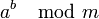
\includegraphics[scale=.6]{graphics/366abde6144a8e6e0d97ba03fd5cde12.png}.

The algorithm must work for any integers \emph{a},\emph{b},\emph{m}
where
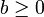
\includegraphics[scale=.6]{graphics/180df89d659ad6dc8f29a74fffe1cfb5.png}
and \emph{m} \textgreater{} 0.



\begin{wideverbatim}

The following function is taken from "lib/rsa.l":

(de **Mod (X Y N)
   (let M 1
      (loop
         (when (bit? 1 Y)
            (setq M (\% (* M X) N)) )
         (T (=0 (setq Y (>> 1 Y)))
            M )
         (setq X (\% (* X X) N)) ) ) )

Test:

: (**Mod
   2988348162058574136915891421498819466320163312926952423791023078876139
   2351399303373464486466122544523690094744975233415544072992656881240319
   10000000000000000000000000000000000000000 )
-> 1527229998585248450016808958343740453059
\end{wideverbatim}

\pagebreak{}
\section*{Monte Carlo methods}

A \textbf{Monte Carlo Simulation} is a way of approximating the value of
a function where calculating the actual value is difficult or
impossible. It uses random sampling to define constraints on the value
and then makes a sort of ``best guess.''

A simple Monte Carlo Simulation can be used to calculate the value for
π. If you had a circle and a square where the length of a side of the
square was the same as the diameter of the circle, the ratio of the area
of the circle to the area of the square would be π/4. So, if you put
this circle inside the square and select many random points inside the
square, the number of points inside the circle divided by the number of
points inside the square and the circle would be approximately π/4.

Write a function to run a simulation like this with a variable number of
random points to select. Also, show the results of a few different
sample sizes. For software where the number π is not built-in, we give π
to a couple of digits: 3.141592653589793238462643383280


\begin{wideverbatim}

(de carloPi (Scl)
   (let (Dim (** 10 Scl)  Dim2 (* Dim Dim)  Pi 0)
      (do (* 4 Dim)
         (let (X (rand 0 Dim)  Y (rand 0 Dim))
            (when (>= Dim2 (+ (* X X) (* Y Y)))
               (inc 'Pi) ) ) )
      (format Pi Scl) ) )

(for N 6
   (prinl (carloPi N)) )

Output:

3.4
3.23
3.137
3.1299
3.14360
3.140964

\end{wideverbatim}

\pagebreak{}
\section*{Monty Hall problem}

Run random simulations of the
\href{http://en.wikipedia.org/wiki/Monty\_Hall\_problem}{Monty Hall}
game. Show the effects of a strategy of the contestant always keeping
his first guess so it can be contrasted with the strategy of the
contestant always switching his guess.

Suppose you're on a game show and you're given the choice of three
doors. Behind one door is a car; behind the others, goats. The car and
the goats were placed randomly behind the doors before the show. The
rules of the game show are as follows: After you have chosen a door, the
door remains closed for the time being. The game show host, Monty Hall,
who knows what is behind the doors, now has to open one of the two
remaining doors, and the door he opens must have a goat behind it. If
both remaining doors have goats behind them, he chooses one randomly.
After Monty Hall opens a door with a goat, he will ask you to decide
whether you want to stay with your first choice or to switch to the last
remaining door. Imagine that you chose Door 1 and the host opens Door 3,
which has a goat. He then asks you ``Do you want to switch to Door
Number 2?'' Is it to your advantage to change your choice?
(\href{http://www.usd.edu/~xtwang/Papers/MontyHallPaper.pdf}{Krauss and
Wang 2003:10})

Note that the player may initially choose any of the three doors (not
just Door 1), that the host opens a different door revealing a goat (not
necessarily Door 3), and that he gives the player a second choice
between the two remaining unopened doors.

Simulate at least a thousand games using three doors for each strategy
and show the results in such a way as to make it easy to compare the
effects of each strategy.


\begin{wideverbatim}

(de montyHall (Keep)
   (let (Prize (rand 1 3)  Choice (rand 1 3))
      (if Keep                    # Keeping the first choice?
         (= Prize Choice)         # Yes: Monty's choice doesn't matter
         (<> Prize Choice) ) ) )  # Else: Win if your first choice was wrong

(prinl
   "Strategy KEEP    -> "
   (let Cnt 0
      (do 10000 (and (montyHall T) (inc 'Cnt)))
      (format Cnt 2) )
   " \%" )

(prinl
   "Strategy SWITCH  -> "
   (let Cnt 0
      (do 10000 (and (montyHall NIL) (inc 'Cnt)))
      (format Cnt 2) )
   " \%" )

Output:

Strategy KEEP    -> 33.01 \%
Strategy SWITCH  -> 67.73 \%

\end{wideverbatim}

\pagebreak{}
\section*{Morse code}

\href{http://en.wikipedia.org/wiki/Morse\_code}{Morse code} is one of
the simplest and most versatile methods of telecommunication in
existence. It has been in use for more than 160 years --- longer than
any other electronic encoding system.

The task: Send a string as audible morse code to an audio device (e.g.,
the PC speaker).

As the standard Morse code does not contain all possible characters, you
may either ignore unknown characters in the file, or indicate them
somehow (e.g. with a different pitch).


\begin{wideverbatim}

The following simply uses the 'beep' pc-speaker beeper utility.

# *Morse *Dit *Dah

(balance '*Morse
   (mapcar
      '((L)
         (def (car L)
            (mapcar = (chop (cadr L)) '("." .)) ) )
      (quote
         ("!"  "---.")     ("\"" ".-..-.")   ("\$" "...-..-")   ("'" ".----.")
         ("(" "-.--.")     (")" "-.--.-")    ("+" ".-.-.")     ("," "--..--")
         ("-" "-....-")    ("." ".-.-.-")    ("/" "-..-.")
         ("0" "-----")     ("1" ".----")     ("2" "..---")     ("3" "...--")
         ("4" "....-")     ("5" ".....")     ("6" "-....")     ("7" "--...")
         ("8" "---..")     ("9" "----.")
         (":" "---...")    (";" "-.-.-.")    ("=" "-...-")     ("?" "..--..")
         ("@" ".--.-.")
         ("A" ".-")        ("B" "-...")      ("C" "-.-.")      ("D" "-..")
         ("E" ".")         ("F" "..-.")      ("G" "--.")       ("H" "....")
         ("I" "..")        ("J" ".---")      ("K" "-.-")       ("L" ".-..")
         ("M" "--")        ("N" "-.")        ("O" "---")       ("P" ".--.")
         ("Q" "--.-")      ("R" ".-.")       ("S" "...")       ("T" "-")
         ("U" "..-")       ("V" "...-")      ("W" ".--")       ("X" "-..-")
         ("Y" "-.--")      ("Z" "--..")
         ("[" "-.--.")     ("]" "-.--.-")    ("_" "..--.-") ) ) )

# Words per minute
(de wpm (N)
   (setq *Dit (*/ 1200 N)  *Dah (* 3 *Dit)) )

(wpm 20)

# Morse a string
(de morse (Str)
   (for C (chop Str)
      (cond
         ((sp? C) (wait (+ *Dah *Dit)))         # White space: Pause
         ((idx '*Morse (uppc C))                # Known character
            (for Flg (val (car @))
               (call "/usr/bin/beep" "-D" *Dit "-l" (if Flg *Dit *Dah)) ) )
         (T (call "/usr/bin/beep" "-f" 370)) )  # Unkown character
      (wait (- *Dah *Dit)) ) )

(morse "Hello world!")

\end{wideverbatim}

\pagebreak{}
\section*{Mouse position}

Get the current location of the mouse cursor relative to the active
window. Please specify if the window may be externally created.


\begin{wideverbatim}

The following works in an XTerm window. After calling (mousePosition), click
into the current terminal window. The returned value is (X . Y), where X is the
column and Y the line number.

(de mousePosition ()
   (prog2
      (prin "^[[?9h")  # Mouse reporting on
      (and
         (= "^[" (key))
         (key 200)
         (key 200)
         (key)
         (cons
            (- (char (key)) 32)
            (- (char (key)) 32) ) )
      (prin "^[[?9l") ) )  # Mouse reporting off

Output:

: (mousePosition)
-> (7 . 3)

\end{wideverbatim}

\pagebreak{}
\section*{Multiline shebang}

Simple shebangs can help with scripting, e.g. \#!/usr/bin/env python at
the top of a Python script will allow it to be run in a terminal as
``./script.py''.

Occasionally, a more complex shebang line is needed. For example, some
languages do not include the program name in ARGV; a multiline shebang
can reorder the arguments so that the program name is included in ARGV.

The syntax for a multiline shebang is complicated. The shebang lines
must be simultaneously commented away from the main language and
revealed to some shell (perhaps \emph{Bash}) so that they can be
executed.

\begin{wideverbatim}

We can use a multi-line comment #{ ... }# to hide the shell commands from Lisp.
The opening #{ in turn is a coment for the shell.

#!/bin/bash
#{
exec pil \$0 foo bar
# }#

# Lisp code
(println (cadr (file)) (opt) (opt))
(bye)

Output:

\$ ./myScript
"myScript" "foo" "bar"

\end{wideverbatim}

\pagebreak{}
\section*{Multiple distinct objects}


Create a \emph{sequence} (array, list, whatever)
consisting of n distinct, initialized items of the same type. n should
be determined at runtime.

By \emph{distinct} we mean that if they are mutable, changes to one do
not affect all others; if there is an appropriate equality operator they
are considered unequal; etc. The code need not specify a particular kind
of distinction, but do not use e.g. a numeric-range generator which does
not generalize.

By \emph{initialized} we mean that each item must be in a well-defined
state appropriate for its type, rather than e.g. arbitrary previous
memory contents in an array allocation. Do not show only an
initialization technique which initializes only to ``zero'' values (e.g.
\texttt{calloc()} or \texttt{int a{[}n{]} = \{\};} in C), unless
user-defined types can provide definitions of ``zero'' for that type.

This task was inspired by the common error of intending to do this, but
instead creating a sequence of n references to the \emph{same} mutable
object; it might be informative to show the way to do that as well, both
as a negative example and as how to do it when that's all that's
actually necessary.

This task is most relevant to languages operating in the
pass-references-by-value style (most object-oriented, garbage-collected,
and/or `dynamic' languages).



\begin{wideverbatim}

Create 5 distinct (empty) objects:

: (make (do 5 (link (new))))
-> (\$384717187 \$384717189 \$384717191 \$384717193 \$384717195)

Create 5 anonymous symbols with the values 1 .. 5:

: (mapcar box (range 1 5))
-> (\$384721107 \$384721109 \$384721111 \$384721113 \$384721115)
: (val (car @))
-> 1
: (val (cadr @@))
-> 2

\end{wideverbatim}

\pagebreak{}
\section*{Multiple regression}


Given a set of data vectors in the following format:

\begin{figure}[H]
\centering
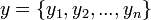
\includegraphics[scale=.6]{graphics/14460313caad694cfeab489628009eab.png}
% \caption{y = \textbackslash{}\{ y\_1, y\_2, ..., y\_n
% \textbackslash{}\}\textbackslash{},}
\end{figure}

\begin{figure}[H]
\centering
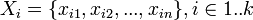
\includegraphics[scale=.6]{graphics/61a7b2eee29145e18a5583d931f62975.png}
% \caption{X\_i = \textbackslash{}\{ x\_\{i1\}, x\_\{i2\}, ..., x\_\{in\}
% \textbackslash{}\}, i \textbackslash{}in 1..k\textbackslash{},}
\end{figure}

Compute the vector β =
\{β\textsubscript{1},β\textsubscript{2},\ldots{},β\textsubscript{\emph{k}}\}
using
\href{http://en.wikipedia.org/wiki/Ordinary\_least\_squares}{ordinary
least squares} regression using the following equation:

\begin{figure}[H]
\centering
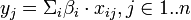
\includegraphics[scale=.6]{graphics/411ee43ddd9e5b42c7ef2ddb2ec7e9fb.png}
% \caption{y\_j = \textbackslash{}Sigma\_i \textbackslash{}beta\_i
% \textbackslash{}cdot x\_\{ij\} , j \textbackslash{}in 1..n}
\end{figure}

You can assume \emph{y} is given to you as a vector (a one-dimensional
array), and \emph{X} is given to you as a two-dimensional array (i.e.
matrix).

\begin{wideverbatim}

(scl 20)

# Matrix transposition
(de matTrans (Mat)
   (apply mapcar Mat list) )

# Matrix multiplication
(de matMul (Mat1 Mat2)
   (mapcar
      '((Row)
         (apply mapcar Mat2
            '(@ (sum */ Row (rest) (1.0 .))) ) )
      Mat1 ) )

# Matrix identity
(de matIdent (N)
   (let L (need N (1.0) 0)
      (mapcar '(() (copy (rot L))) L) ) )

# Reduced row echelon form
(de reducedRowEchelonForm (Mat)
   (let (Lead 1  Cols (length (car Mat)))
      (for (X Mat X (cdr X))
         (NIL
            (loop
               (T (seek '((R) (n0 (get R 1 Lead))) X)
                  @ )
               (T (> (inc 'Lead) Cols)) ) )
         (xchg @ X)
         (let D (get X 1 Lead)
            (map
               '((R) (set R (*/ (car R) 1.0 D)))
               (car X) ) )
         (for Y Mat
            (unless (== Y (car X))
               (let N (- (get Y Lead))
                  (map
                     '((Dst Src)
                        (inc Dst (*/ N (car Src) 1.0)) )
                     Y
                     (car X) ) ) ) )
         (T (> (inc 'Lead) Cols)) ) )
   Mat )

\end{wideverbatim}

\begin{wideverbatim}


(de matInverse (Mat)
   (let N (length Mat)
      (unless (= N (length (car Mat)))
         (quit "can't invert a non-square matrix") )
      (mapc conc Mat (matIdent N))
      (mapcar '((L) (tail N L)) (reducedRowEchelonForm Mat)) ) )

(de columnVector (Ary)
   (mapcar cons Ary) )

(de regressionCoefficients (Mat X)
   (let Xt (matTrans X)
      (matMul (matMul (matInverse (matMul Xt X)) Xt) Mat) ) )

(setq
   Y (columnVector (1.0 2.0 3.0 4.0 5.0))
   X (columnVector (2.0 1.0 3.0 4.0 5.0)) )

(round (caar (regressionCoefficients Y X)) 17)

Output:

-> "0.98181818181818182"

\end{wideverbatim}

\pagebreak{}
\section*{Multiplication tables}

Produce a formatted 12×12 multiplication table of the kind memorised by
rote when in primary school.

Only print the top half triangle of products.


\begin{wideverbatim}

(de mulTable (N)
   (space 4)
   (for X N
      (prin (align 4 X)) )
   (prinl)
   (prinl)
   (for Y N
      (prin (align 4 Y))
      (space (* (dec Y) 4))
      (for (X Y (>= N X) (inc X))
         (prin (align 4 (* X Y))) )
      (prinl) ) )

(mulTable 12)

Output:

       1   2   3   4   5   6   7   8   9  10  11  12

   1   1   2   3   4   5   6   7   8   9  10  11  12
   2       4   6   8  10  12  14  16  18  20  22  24
   3           9  12  15  18  21  24  27  30  33  36
   4              16  20  24  28  32  36  40  44  48
   5                  25  30  35  40  45  50  55  60
   6                      36  42  48  54  60  66  72
   7                          49  56  63  70  77  84
   8                              64  72  80  88  96
   9                                  81  90  99 108
  10                                     100 110 120
  11                                         121 132
  12                                             144

\end{wideverbatim}

\pagebreak{}
\section*{Multisplit}

It is often necessary to split a string into pieces based on several
different (potentially multi-character) separator strings, while still
retaining the information about which separators were present in the
input. This is particularly useful when doing small parsing tasks. The
task is to write code to demonstrate this.

The function (or procedure or method, as appropriate) should take an
input string and an ordered collection of separators. The order of the
separators is significant: The delimiter order represents priority in
matching, with the first defined delimiter having the highest priority.
In cases where there would be an ambiguity as to which separator to use
at a particular point (e.g., because one separator is a prefix of
another) the separator with the highest priority should be used.
Delimiters can be reused and the output from the function should be an
ordered sequence of substrings.

Test your code using the input string ``\texttt{a!===b=!=c}'' and the
separators ``\texttt{==}'', ``\texttt{!=}'' and ``\texttt{=}''.

For these inputs the string should be parsed as
\texttt{"a" (!=) "" (==) "b" (=) "" (!=) "c"}, where matched delimiters
are shown in parentheses, and separated strings are quoted, so our
resulting output is \texttt{"a", empty string, "b", empty string, "c"}.
Note that the quotation marks are shown for clarity and do not form part
of the output.

\textbf{Extra Credit:} provide information that indicates which
separator was matched at each separation point and where in the input
string that separator was matched.


\begin{wideverbatim}

(de multisplit (Str Sep)
   (setq Sep (mapcar chop Sep))
   (make
      (for (S (chop Str) S)
         (let L
            (make
               (loop
                  (T (find head Sep (circ S))
                     (link
                        (list
                           (- (length Str) (length S))
                           (pack (cut (length @) 'S)) ) ) )
                  (link (pop 'S))
                  (NIL S (link NIL)) ) )
            (link (pack (cdr (rot L))))
            (and (car L) (link @)) ) ) ) )

(println (multisplit "a!===b=!=c" '("==" "!=" "=")))
(println (multisplit "a!===b=!=c" '("=" "!=" "==")))

Output:

("a" (1 "!=") NIL (3 "==") "b" (6 "=") NIL (7 "!=") "c")
("a" (1 "!=") NIL (3 "=") NIL (4 "=") "b" (6 "=") NIL (7 "!=") "c")

\end{wideverbatim}

\pagebreak{}
\section*{Mutex}

A \textbf{mutex} (\emph{abbreviated} \textbf{Mut}ually
\textbf{Ex}clusive access) is a synchronization object, a variant of
\emph{semaphore} with \emph{k}=1. A mutex is said to be
seized by a \emph{task} decreasing \emph{k}. It is released
when the task restores \emph{k}. Mutexes are typically used to protect a
shared resource from concurrent access. A \emph{task} seizes
(or acquires) the mutex, then accesses the resource, and after that
releases the mutex.

A mutex is a low-level synchronization primitive exposed to deadlocking.
A deadlock can occur with just two tasks and two mutexes (if each task
attempts to acquire both mutexes, but in the opposite order). Entering
the deadlock is usually aggravated by a
\emph{race condition} state, which leads to
sporadic hangups, which are very difficult to track down.


\begin{wideverbatim}

PicoLisp uses several mechanisms of interprocess communication, mainly within
the same process family (children of the same parent process) for database
synchronization (e.g.
'[http://software-lab.de/doc/refL.html#lock lock]',
'[http://software-lab.de/doc/refS.html#sync sync]' or
'[http://software-lab.de/doc/refT.html#tell tell]'.

For a simple synchronization of unrelated PicoLisp processes the
'[http://software-lab.de/doc/refA.html#acquire acquire]' /
'[http://software-lab.de/doc/refR.html#release release]' function pair
can be used.

\end{wideverbatim}

\pagebreak{}
\section*{Mutual recursion}

Two functions are said to be mutually recursive if the first calls the
second, and in turn the second calls the first.

Write two mutually recursive functions that compute members of the
\href{http://en.wikipedia.org/wiki/Hofstadter\_sequence\#Hofstadter\_Female\_and\_Male\_sequences}{Hofstadter
  Female and Male sequences} defined as:

\begin{figure}[H]
\centering
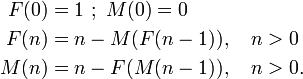
\includegraphics[scale=.6]{graphics/af460b7986d4afc5fe920b86f15f522a.png}
% \caption{ \textbackslash{}begin\{align\}
% F(0)\&=1\textbackslash{}~;\textbackslash{} M(0)=0
% \textbackslash{}\textbackslash{} F(n)\&=n-M(F(n-1)),
% \textbackslash{}quad n\textgreater{}0 \textbackslash{}\textbackslash{}
% M(n)\&=n-F(M(n-1)), \textbackslash{}quad n\textgreater{}0.
% \textbackslash{}end\{align\} }
\end{figure}

(If a language does not allow for a solution using mutually recursive
functions then state this rather than give a solution by other means).


\begin{wideverbatim}

(de f (N)
   (if (=0 N)
      1
      (- N (m (f (dec N)))) ) )

(de m (N)
   (if (=0 N)
      0
      (- N (f (m (dec N)))) ) )

\end{wideverbatim}



% %%%%%%%%%%%%%%%%%%%%%%%% referenc.tex %%%%%%%%%%%%%%%%%%%%%%%%%%%%%%
% sample references
% %
% Use this file as a template for your own input.
%
%%%%%%%%%%%%%%%%%%%%%%%% Springer-Verlag %%%%%%%%%%%%%%%%%%%%%%%%%%
%
% BibTeX users please use
% \bibliographystyle{}
% \bibliography{}
%
\biblstarthook{In view of the parallel print and (chapter-wise) online publication of your book at \url{www.springerlink.com} it has been decided that -- as a genreral rule --  references should be sorted chapter-wise and placed at the end of the individual chapters. However, upon agreement with your contact at Springer you may list your references in a single seperate chapter at the end of your book. Deactivate the class option \texttt{sectrefs} and the \texttt{thebibliography} environment will be put out as a chapter of its own.\\\indent
References may be \textit{cited} in the text either by number (preferred) or by author/year.\footnote{Make sure that all references from the list are cited in the text. Those not cited should be moved to a separate \textit{Further Reading} section or chapter.} The reference list should ideally be \textit{sorted} in alphabetical order -- even if reference numbers are used for the their citation in the text. If there are several works by the same author, the following order should be used: 
\begin{enumerate}
\item all works by the author alone, ordered chronologically by year of publication
\item all works by the author with a coauthor, ordered alphabetically by coauthor
\item all works by the author with several coauthors, ordered chronologically by year of publication.
\end{enumerate}
The \textit{styling} of references\footnote{Always use the standard abbreviation of a journal's name according to the ISSN \textit{List of Title Word Abbreviations}, see \url{http://www.issn.org/en/node/344}} depends on the subject of your book:
\begin{itemize}
\item The \textit{two} recommended styles for references in books on \textit{mathematical, physical, statistical and computer sciences} are depicted in ~\cite{science-contrib, science-online, science-mono, science-journal, science-DOI} and ~\cite{phys-online, phys-mono, phys-journal, phys-DOI, phys-contrib}.
\item Examples of the most commonly used reference style in books on \textit{Psychology, Social Sciences} are~\cite{psysoc-mono, psysoc-online,psysoc-journal, psysoc-contrib, psysoc-DOI}.
\item Examples for references in books on \textit{Humanities, Linguistics, Philosophy} are~\cite{humlinphil-journal, humlinphil-contrib, humlinphil-mono, humlinphil-online, humlinphil-DOI}.
\item Examples of the basic Springer style used in publications on a wide range of subjects such as \textit{Computer Science, Economics, Engineering, Geosciences, Life Sciences, Medicine, Biomedicine} are ~\cite{basic-contrib, basic-online, basic-journal, basic-DOI, basic-mono}. 
\end{itemize}
}

\begin{thebibliography}{99.}%
% and use \bibitem to create references.
%
% Use the following syntax and markup for your references if 
% the subject of your book is from the field 
% "Mathematics, Physics, Statistics, Computer Science"
%
% Contribution 
\bibitem{science-contrib} Broy, M.: Software engineering --- from auxiliary to key technologies. In: Broy, M., Dener, E. (eds.) Software Pioneers, pp. 10-13. Springer, Heidelberg (2002)
%
% Online Document
\bibitem{science-online} Dod, J.: Effective substances. In: The Dictionary of Substances and Their Effects. Royal Society of Chemistry (1999) Available via DIALOG. \\
\url{http://www.rsc.org/dose/title of subordinate document. Cited 15 Jan 1999}
%
% Monograph
\bibitem{science-mono} Geddes, K.O., Czapor, S.R., Labahn, G.: Algorithms for Computer Algebra. Kluwer, Boston (1992) 
%
% Journal article
\bibitem{science-journal} Hamburger, C.: Quasimonotonicity, regularity and duality for nonlinear systems of partial differential equations. Ann. Mat. Pura. Appl. \textbf{169}, 321--354 (1995)
%
% Journal article by DOI
\bibitem{science-DOI} Slifka, M.K., Whitton, J.L.: Clinical implications of dysregulated cytokine production. J. Mol. Med. (2000) doi: 10.1007/s001090000086 
%
\bigskip

% Use the following (APS) syntax and markup for your references if 
% the subject of your book is from the field 
% "Mathematics, Physics, Statistics, Computer Science"
%
% Online Document
\bibitem{phys-online} J. Dod, in \textit{The Dictionary of Substances and Their Effects}, Royal Society of Chemistry. (Available via DIALOG, 1999), 
\url{http://www.rsc.org/dose/title of subordinate document. Cited 15 Jan 1999}
%
% Monograph
\bibitem{phys-mono} H. Ibach, H. L\"uth, \textit{Solid-State Physics}, 2nd edn. (Springer, New York, 1996), pp. 45-56 
%
% Journal article
\bibitem{phys-journal} S. Preuss, A. Demchuk Jr., M. Stuke, Appl. Phys. A \textbf{61}
%
% Journal article by DOI
\bibitem{phys-DOI} M.K. Slifka, J.L. Whitton, J. Mol. Med., doi: 10.1007/s001090000086
%
% Contribution 
\bibitem{phys-contrib} S.E. Smith, in \textit{Neuromuscular Junction}, ed. by E. Zaimis. Handbook of Experimental Pharmacology, vol 42 (Springer, Heidelberg, 1976), p. 593
%
\bigskip
%
% Use the following syntax and markup for your references if 
% the subject of your book is from the field 
% "Psychology, Social Sciences"
%
%
% Monograph
\bibitem{psysoc-mono} Calfee, R.~C., \& Valencia, R.~R. (1991). \textit{APA guide to preparing manuscripts for journal publication.} Washington, DC: American Psychological Association.
%
% Online Document
\bibitem{psysoc-online} Dod, J. (1999). Effective substances. In: The dictionary of substances and their effects. Royal Society of Chemistry. Available via DIALOG. \\
\url{http://www.rsc.org/dose/Effective substances.} Cited 15 Jan 1999.
%
% Journal article
\bibitem{psysoc-journal} Harris, M., Karper, E., Stacks, G., Hoffman, D., DeNiro, R., Cruz, P., et al. (2001). Writing labs and the Hollywood connection. \textit{J Film} Writing, 44(3), 213--245.
%
% Contribution 
\bibitem{psysoc-contrib} O'Neil, J.~M., \& Egan, J. (1992). Men's and women's gender role journeys: Metaphor for healing, transition, and transformation. In B.~R. Wainrig (Ed.), \textit{Gender issues across the life cycle} (pp. 107--123). New York: Springer.
%
% Journal article by DOI
\bibitem{psysoc-DOI}Kreger, M., Brindis, C.D., Manuel, D.M., Sassoubre, L. (2007). Lessons learned in systems change initiatives: benchmarks and indicators. \textit{American Journal of Community Psychology}, doi: 10.1007/s10464-007-9108-14.
%
%
% Use the following syntax and markup for your references if 
% the subject of your book is from the field 
% "Humanities, Linguistics, Philosophy"
%
\bigskip
%
% Journal article
\bibitem{humlinphil-journal} Alber John, Daniel C. O'Connell, and Sabine Kowal. 2002. Personal perspective in TV interviews. \textit{Pragmatics} 12:257--271
%
% Contribution 
\bibitem{humlinphil-contrib} Cameron, Deborah. 1997. Theoretical debates in feminist linguistics: Questions of sex and gender. In \textit{Gender and discourse}, ed. Ruth Wodak, 99--119. London: Sage Publications.
%
% Monograph
\bibitem{humlinphil-mono} Cameron, Deborah. 1985. \textit{Feminism and linguistic theory.} New York: St. Martin's Press.
%
% Online Document
\bibitem{humlinphil-online} Dod, Jake. 1999. Effective substances. In: The dictionary of substances and their effects. Royal Society of Chemistry. Available via DIALOG. \\
http://www.rsc.org/dose/title of subordinate document. Cited 15 Jan 1999
%
% Journal article by DOI
\bibitem{humlinphil-DOI} Suleiman, Camelia, Daniel C. O�Connell, and Sabine Kowal. 2002. `If you and I, if we, in this later day, lose that sacred fire...�': Perspective in political interviews. \textit{Journal of Psycholinguistic Research}. doi: 10.1023/A:1015592129296.
%
%
%
\bigskip
%
%
% Use the following syntax and markup for your references if 
% the subject of your book is from the field 
% "Computer Science, Economics, Engineering, Geosciences, Life Sciences"
%
%
% Contribution 
\bibitem{basic-contrib} Brown B, Aaron M (2001) The politics of nature. In: Smith J (ed) The rise of modern genomics, 3rd edn. Wiley, New York 
%
% Online Document
\bibitem{basic-online} Dod J (1999) Effective Substances. In: The dictionary of substances and their effects. Royal Society of Chemistry. Available via DIALOG. \\
\url{http://www.rsc.org/dose/title of subordinate document. Cited 15 Jan 1999}
%
% Journal article by DOI
\bibitem{basic-DOI} Slifka MK, Whitton JL (2000) Clinical implications of dysregulated cytokine production. J Mol Med, doi: 10.1007/s001090000086
%
% Journal article
\bibitem{basic-journal} Smith J, Jones M Jr, Houghton L et al (1999) Future of health insurance. N Engl J Med 965:325--329
%
% Monograph
\bibitem{basic-mono} South J, Blass B (2001) The future of modern genomics. Blackwell, London 
%
\end{thebibliography}

